%%%%%%%%%%%%%%%%%%%%%%%%%%%%%%%%%%%%%%%%%
% University Assignment Title Page 
% LaTeX Template
% Version 1.0 (27/12/12)
%
% This template has been downloaded from:
% http://www.LaTeXTemplates.com
%
% Original author:
% WikiBooks (http://en.wikibooks.org/wiki/LaTeX/Title_Creation)
%
% License:
% CC BY-NC-SA 3.0 (http://creativecommons.org/licenses/by-nc-sa/3.0/)
% 
% Instructions for using this template:
% This title page is capable of being compiled as is. This is not useful for 
% including it in another document. To do this, you have two options: 
%
% 1) Copy/paste everything between \begin{document} and \end{document} 
% starting at \begin{titlepage} and paste this into another LaTeX file where you 
% want your title page.
% OR
% 2) Remove everything outside the \begin{titlepage} and \end{titlepage} and 
% move this file to the same directory as the LaTeX file you wish to add it to. 
% Then add \input{./title_page_1.tex} to your LaTeX file where you want your
% title page.
%
%%%%%%%%%%%%%%%%%%%%%%%%%%%%%%%%%%%%%%%%%
%\title{Title page with logo}
%----------------------------------------------------------------------------------------
%	PACKAGES AND OTHER DOCUMENT CONFIGURATIONS
%----------------------------------------------------------------------------------------

\documentclass[12pt]{article}
\usepackage[english]{babel}
\usepackage[utf8x]{inputenc}
\usepackage{amsmath}
\usepackage{graphicx}
\usepackage[colorinlistoftodos]{todonotes}
\usepackage{multirow}
\usepackage{enumerate}

\begin{document}

\begin{titlepage}

\newcommand{\HRule}{\rule{\linewidth}{0.5mm}} % Defines a new command for the horizontal lines, change thickness here

\center % Center everything on the page
 
%----------------------------------------------------------------------------------------
%	HEADING SECTIONS
%----------------------------------------------------------------------------------------

\textsc{\LARGE University of California, Irvine}\\[1.5cm] % Name of your university/college
\textsc{\Large Introduction to Artificial Intelligence}\\[0.5cm] % Major heading such as course name
\textsc{\large CompSci 271, Fall 2016}\\[0.5cm] % Minor heading such as course title

%----------------------------------------------------------------------------------------
%	TITLE SECTION
%----------------------------------------------------------------------------------------

\HRule \\[0.4cm]
{ \huge \bfseries Sudoku Solver}\\[0.4cm] % Title of your document
\HRule \\[1.5cm]
 
%----------------------------------------------------------------------------------------
%	AUTHOR SECTION
%----------------------------------------------------------------------------------------

\begin{minipage}{0.4\textwidth}
\begin{flushleft} \large
\emph{Author:}\\
Liangjian Chen \\% Your name
Yu Guo \\
Shengnan Wang \\
Shutao Xiao
\end{flushleft}
\end{minipage}
~
\begin{minipage}{0.4\textwidth}
\begin{flushright} \large
\emph{Instructor:} \\
Dr. Kalev Kask % Supervisor's Name
\end{flushright}
\end{minipage}\\[2cm]

% If you don't want a supervisor, uncomment the two lines below and remove the section above
%\Large \emph{Author:}\\
%John \textsc{Smith}\\[3cm] % Your name

%----------------------------------------------------------------------------------------
%	DATE SECTION
%----------------------------------------------------------------------------------------

{\large \today}\\[2cm] % Date, change the \today to a set date if you want to be precise

%----------------------------------------------------------------------------------------
%	LOGO SECTION
%----------------------------------------------------------------------------------------

% \includegraphics{logo.png}\\[1cm] % Include a department/university logo - this will require the graphicx package
 
%----------------------------------------------------------------------------------------

\vfill % Fill the rest of the page with whitespace

\end{titlepage}


% \begin{abstract}
% Your abstract.
% \end{abstract}


\section{Introduction}
	Sudoku, in Japanese, means Number place, and it is one of the most popular number games since 2005. 
	To solve Sudoku, one needs to use a logic-based combination and trial and error. 

	\begin{figure}[ht]
	\centering
	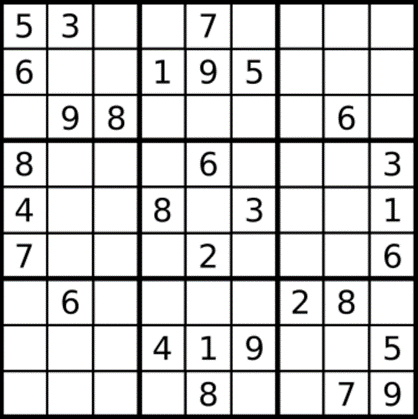
\includegraphics[width=0.5\textwidth]{figure/sudoku1.png}
	\caption{An example of Sudoku problem}
	\label{fig:sudoku1}
	\end{figure}

	As is shown in Figure \ref{fig:sudoku1}, a Sudoku board contains 81 squares, and some of the squares are initially filled with digits from 1 to 9.
	Given this partially filled $9 \times 9$ board, one needs to fill all empty grids.
	The rules is that no digit appears twice in any row, column, or $3 \times 3$ box.  
	The result of this Sudoku is shown in Figure \ref{fig:sudoku2}.  

	\begin{figure}[ht]
	\centering
	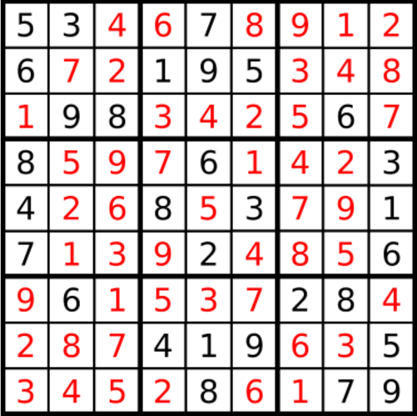
\includegraphics[width=0.5\textwidth]{figure/sudoku2.png}
	\caption{An solution of Sudoku in Figure \ref{fig:sudoku1}}
	\label{fig:sudoku2}
	\end{figure}

	The basic idea to solve the Sudoku is using the depth-first search (DFS) with backtracking. 
	Although Sudoku is a completed game and it is just involved 81 squares, there are 6,670,903,752,021,072,936,960 valid Sudoku grids.  
	Hence, for some difficult Sudoku problem, it is too slow to use the basic DFS algorithm. 
	In this report, two algorithms are mainly discussed to solve the Sudoku problem: one is DFS with the optimization, such as constraint propagation and heuristics, the other is dancing links algorithm. 
	In next section, these methods will be introduced in detail.  
	The implementation and results will be discussed in the last section.


\section{Method}

	\subsection{Constraint satisfaction problem (CSP)}
		A Sudoku puzzle could be considered as a CSP with 81 variables and one square is one variable. 
		Obviously, the domains of variables are the digits from 1 to 9. 
		As is shown in Figure \ref{fig:sudoku3}, the names of 81 variables could be $A1$ through $A9$ for the top row (left to right), down to $I1$ through $I9$ for the bottom row. 
		A row, column, or box is called a unit. 
		What’s more, there are 27 different constraints: 9 for row, 9 for column and 9 for $3 \times 3$ box:

		\begin{gather*}
		\mathit{Alldiff}(A1, A2, A3, A4, A5, A6, A7, A8, A9) \\
		\mathit{Alldiff}(B1, B2, B3, B4, B5, B6, B7, B8, B9) \\
		\dots \\
		\mathit{Alldiff}(A1, B1, C1, D1, E1, F1, G1, H1, I1) \\
		\mathit{Alldiff}(A2, B2, C2, D2, E2, F2, G2, H2, I2) \\
		\dots \\
		\mathit{Alldiff}(A1, A2, A3, B1, B2, B3, C1, C2, C3) \\
		\mathit{Alldiff}(A4, A5, A6, B4, B5, B6, C4, C5, C6) \\
		\dots
		\end{gather*}

		\begin{figure}[ht]
		\centering
		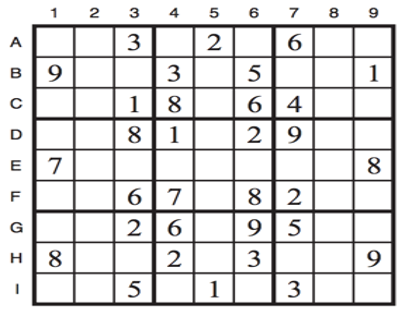
\includegraphics[width=0.5\textwidth]{figure/sudoku3.png}
		\caption{The names of variable of Sudoku puzzle as CSP}
		\label{fig:sudoku3}
		\end{figure}

	\subsection{Backtracking}
		As mentioned above, the direct method to solve the Sudoku problem is backtracking search which is a kind of DFS: 
		one picks the first empty square and assign one and then check whether there is any conflict. 
		If there is not, do the same procedure for the second empty square. 
		If there is conflict, then assign two to the first square. 
		So the basic idea of backtracking is that if there is no conflict, then choose the next variable and assign a value for it. 
		If there is no possible value for the square, then return to previous square and re-assign another value. 
		It is known that backtracking search is a complete algorithm and it is guaranteed to find a solution if there exist a solution, 
		since, every possible states are taken into consideration during backtracking search. 
		For Sudoku, there are roughly $9^{81-n}$ states to be search ($n$ is the filled squares in the given board) and we could reduced the number of the states to be searched by some strategy. 
		Constraint propagation, minimum-remaining-value and least-constraining-value heuristic are adopted in our project.

		\subsubsection{Constraint propagation}
			Constraint propagation is a specific type of inference of CSP: 
			we use the constraint to decrease the number of legal values for a variable, which in turn could reduce the legal values for another variable, and so on. 
			In the project, two kinds of constraint propagation are implemented. 
			First, if the square $M$ has only one value, then remove this value from the domain of other 20 squares in the same row, column and $3 \times 3$ box with $M$. 
			Second, if a unit (one row, column or $3 \times 3$ box) has only one place for the value, then put the value in that place. 
			Taken the second row as an example: in the second row, $B1$ already is filled with 2, and we know that from $B3$ to $B9$, there is no 3 in their domain. Hence, $B2$ should be filled with 3. 

		\subsubsection{Minimum-remaining-value (MRV) heuristic}
			In order to determine the order of the variable to be assigned, minimum-remaining-value heuristic is adopted. 
			It means that we choose the most constrained variable, i.e, choose the variable with the fewest legal values. 
			The MRV heuristic usually performs better than a random or static ordering, sometimes by a factor of 1,000 or more, although the results vary widely depending on the problem. (RV page 216).

		\subsubsection{Least-constraining-value heuristic}
			Aftering determining the variable $M$ which is the variable to be taken into consideration, which values should be chosen from the domain of $M$?
			Here, another heuristic-least-constraining-value (LCV) is used to assign value for a variable. 
			Specifically,  we choose the value that rules out the fewest values in the remaining variables, 
			that is to say, leave more space for the rest variables. 
			In general, the heuristic is trying to leave the maximum flexibility for subsequent variable assignments.

	\subsection{Algorithm X with Dance-Link (DLX)}
		Dancing Links is an algorithm by Knuth to solve Exact Cover Problems (also called Algorithm X). 
		Algorithm X is a recursive, nondeterministic, depth-first, backtracking algorithm that finds all solutions to the exact cover problem. 
		An exact cover problem, for our purposes, is as follows: given a matrix of ones and zeros, select a subset $S$ of the rows so that each column has exactly one \textbf{1} when looking at just the rows $S$.

		What’s important for us, is that a Sudoku puzzle can be trivially represented as an Exact Cover Problem. 
		Not only that, but many other problems, when suitably expressed as an exact cover problem (for example N-queens), can also be solved using Algorithm X. We just need to write Algorithm X once, and then for any problem in which we are interested in and which can be formulate as an exact cover problem, we just need to implement the translation.

		To create the sparse matrix of Sudoku needed to convert the problem into an Exact Cover Problem, we need to recognize what the rows and columns represent. The columns represent the constraints of the puzzle. In Sudoku, we have:

		\begin{enumerate}
		\item A position constraint: Only 1 number can occupy a cell
		\item A row constraint: Only 1 instance of a number can be in the row
		\item A column constraint: Only 1 instance of a number can be in a column
		\item A region constraint: Only 1 instance of a number can be in a region
		\end{enumerate}

		Each number comes with its own set of constraints. Therefore there are $4 \times$ SIZE$^2$ columns., where SIZE is the number of candidates/rows/cols there are in the Sudoku Puzzle. In a $9 \times 9$, this would be 324 columns.

		The rows represent every single possible position for every number. Therefore, there are SIZE$^3$ rows. In a $9 \times 9$, this would be 729 rows. Each row would represent only one candidate position. Therefore, only 9 \textbf{1}s will be in the row, representing the constraints of that position. See Figure \ref{fig:DLX}

		\begin{figure}[ht]
		\centering
		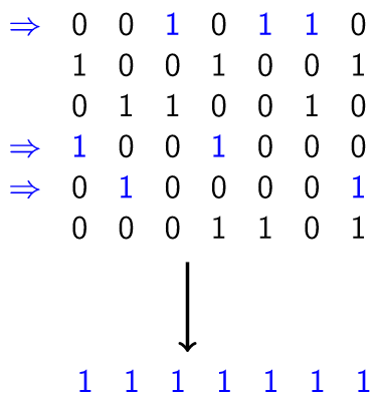
\includegraphics[width=0.5\textwidth]{figure/DLX.png}
		\caption{All columns is covered}
		\label{fig:DLX}
		\end{figure}

		Given initial positions in the matrix, those rows will be included in the answer and covered. Then the Search algorithm will produce the solutions to the puzzle.



\section{Results and Conclusion}

	For now, we have two methods to solve Sudoku problem, CSP with heuristic and DLX. 
	In this section, we are comparing our methods with Na\"\i{}ve method in Ubuntu 14.04 with Intel Quad Core Q9400 (2.66GHz) and 8G memory.
	In Figure \ref{fig:time}, we tested more than 300 cases with various inputs in different difficulty levels. From left to right, the difficulty level of Sudoku game increased. Problem No.1-100 are super easy; problem No.101-200 are at decent level; and problem No.201-300 are nightmares for human.

	\begin{figure}[ht]
	\centering
	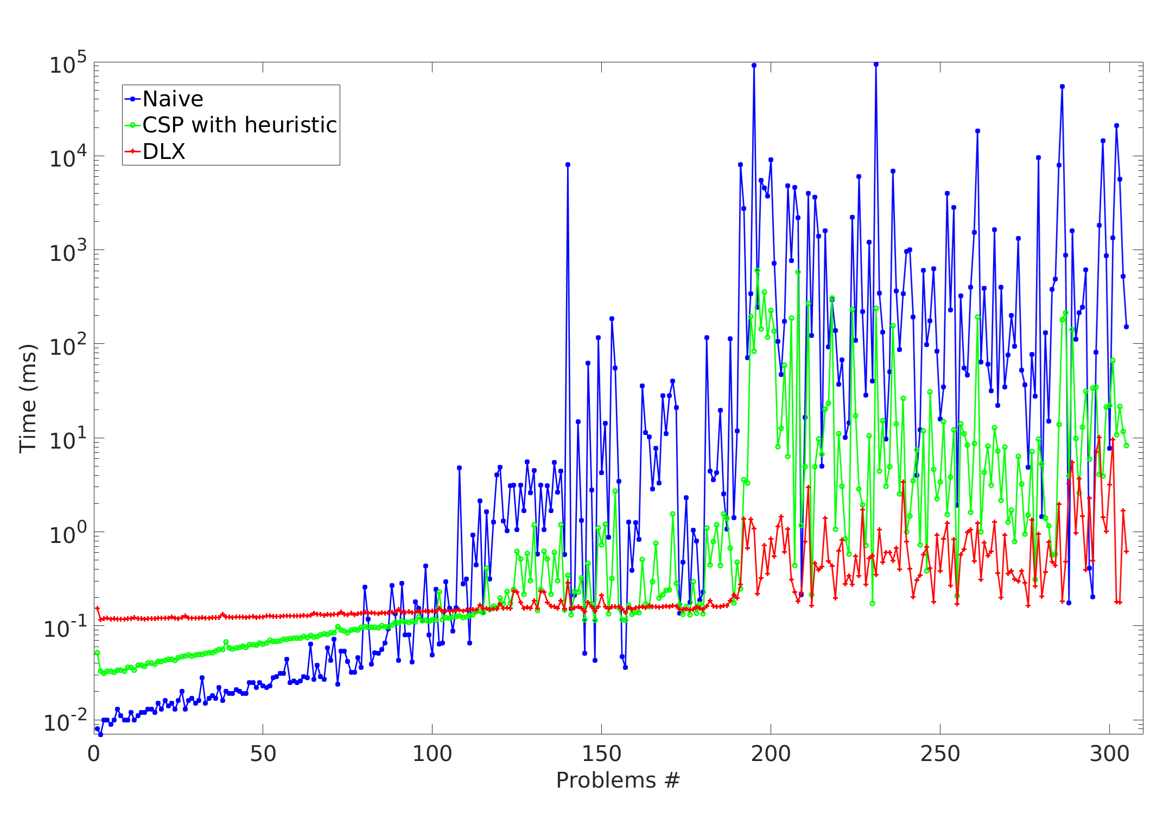
\includegraphics[width=\textwidth]{figure/time.png}
	\caption{Efficiency of different methods}
	\label{fig:time}
	\end{figure}

	Because it needs time to build Dancing Links data structures, using DLX to find a solution is a little slower than the others. 
	But as the perceived difficulty-level increased, the DLX solver performed much better. 
	Solving a board takes on average below a millisecond with DLX. As a rough estimate, DLX is around 10 to 100 times faster (including the time to perform the translation and set-up of Dancing Links data structures).


	\subsection{Benchmark}
		For each difficulty setting (easy, medium, hard, evil), 8 boards were offered by Professor and then used for benchmarking.
		Table \ref{tab:benchmark} below shows results (in milliseconds).

		\begin{table}[ht]
		\centering
		\caption{Benchmark}
		\label{tab:benchmark}
		\begin{tabular}{|l|l|l|l|l|l|l|l|l|}
		\hline
		\multirow{2}{*}{} & \multicolumn{1}{c|}{Easy} & \multicolumn{2}{c|}{Medium} & \multicolumn{2}{c|}{Hard} & \multicolumn{3}{c|}{Evil} \\
		 				\cline{2-9} 
		                  & \multicolumn{1}{c|}{\#1}  & \multicolumn{1}{c|}{\#2} & \multicolumn{1}{c|}{\#3} & \multicolumn{1}{c|}{\#4} & \multicolumn{1}{c|}{\#5} & \multicolumn{1}{c|}{\#6} & \multicolumn{1}{c|}{\#7} & \multicolumn{1}{c|}{\#8} \\ 
		                \hline
		Na\"\i{}ve  & 0.335 & 2.020 & 0.835 & 0.880 & 1.706 & 9.788 & 77.694 & 1.423 \\ 
		\hline
		CSP  & 0.157 & 0.319 & 0.167 & 0.152 & 0.202 & 1.266 & 0.207 & 0.208 \\ 
		\hline
		DLX  & 0.191 & 0.153 & 0.154 & 0.159 & 0.160 & 0.208 & 0.191 & 0.165 \\
		\hline
		\end{tabular}
		\end{table}



\section{Reference}

	\begin{enumerate}[{[1]}]
	\item S. Russell and P. Norvig, "Artificial Intelligence: A Modern Approach" (Third Edition), Prentice Hall, 2009
	\item Knuth Donald, "Dancing links". Millennial Perspectives in Computer Science. P159,187, 2000
	\item Felgenhauer, Bertram and Frazer Jarvis. “Enumerating possible Sudoku grids.” 2005, 2009
	\item http://norvig.com/sudoku.html
	\item https://en.wikipedia.org/wiki/Sudoku
	\end{enumerate}

\end{document}